%This is a Latex file.
\documentclass[12pt]{article}
\usepackage{latexsym,fancyhdr,amsmath,amsfonts,amsthm,dsfont}
\usepackage{amssymb}
\usepackage{tikz}

% margins are relative to the default of 1 in
%\topmargin       -0.2 in

\topmargin        -0.2 in
\textheight       8.4 in
\oddsidemargin    0 in     % this is for pages 1, 3, 5, ...
\evensidemargin   0 in     % and this for 2, 4, 6, ...
\textwidth        6.5 in
%\headheight       15 in     % we won't have a running head, nor
\headsep          .35 in     % any extra space between head and text

%\parindent 0pt

\pagestyle{fancy} \lhead{\sf MTH 317} \chead{\sf Homework 2}
\rhead{\sf Rayana Gottschall} \lfoot{} \cfoot{} \rfoot{}

\newcommand{\C}{\mathds{C}}
\newcommand{\I}{\mathds{I}}
\newcommand{\N}{\mathds{N}}
\newcommand{\Q}{\mathds{Q}}
\newcommand{\R}{\mathds{R}}
\newcommand{\Z}{\mathds{Z}}

\begin{document}
\begin{enumerate}
\item[1.22] .

    \begin{proof}
    rtete
    \end{proof}
    
\item[1.24] Determine whether the graphs $G_1$ and $G_2$ are bipartite. If a graph is bipartite, then redraw it indicating the 
    partite sets; if not, then give an explanation as to why the graph is not bipartite.
\item[$G_1$]
    \begin{center}
    $G_2$ is not bipartite because it contains at least one odd cycle of order 5. 
    \begin{tikzpicture}[scale=1, every node/.style={circle, draw, fill=white, inner sep=2pt}]
    \node ($r_1$) at (0,5) {};
    \node ($q_1$) at (0,4) {};
    \node ($u_1$) at (0,3) {};
    \node ($y_1$) at (0,2) {};
    \node ($w_1$) at (0,1) {};
    \node ($t_1$) at (0,0) {};
    \node ($x_1$) at (2,5) {};
    \node ($v_1$) at (2,4) {};
    \node ($z_1$) at (2,3) {};
    \node ($s_1$) at (2,2) {};

    \draw ($r_1$) -- ($x_1$);
    \draw ($q_1$) -- ($x_1$);
    \draw ($u_1$) -- ($x_1$);
    \draw ($u_1$) -- ($v_1$);
    \draw ($u_1$) -- ($z_1$);
    \draw ($y_1$) -- ($x_1$);
    \draw ($y_1$) -- ($z_1$);
    \draw ($w_1$) -- ($x_1$);
    \draw ($w_1$) -- ($v_1$);
    \draw ($w_1$) -- ($z_1$);
    \draw ($w_1$) -- ($s_1$);
    \draw ($t_1$) -- ($z_1$);
    \draw ($t_1$) -- ($s_1$);
    \end{tikzpicture}
    \end{center}
\item[$G_2$]
    \begin{center}
    $G_2$ is not bipartite because it contains at least one odd cycle of order 5. 
    \begin{tikzpicture}[scale=1, every node/.style={circle, draw, fill=white, inner sep=2pt}]
    \node (A) at (0,0) {};
    \node (B) at (0,3) {};
    \node (C) at (0,5) {};
    \node (D) at (2,-3) {};
    \node (E) at (4,-3) {};

    \draw (A) -- (B);
    \draw (A) -- (D);
    \draw (B) -- (C);
    \draw (C) -- (E);
    \draw (D) -- (E);
    \end{tikzpicture}
    \end{center}

 \item[1.33]
 
\item[2.4] Give an example of a Graph $G$ of order 6 and size 10 such that $\partial$(G) = 3 and $\Delta$(G) = 4.
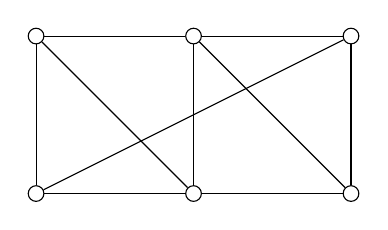
\begin{tikzpicture}[scale=1, every node/.style={circle, draw, fill=white, inner sep=2pt}]
    \node (A) at (0,0) {};
    \node (B) at (2,0) {};
    \node (C) at (2,2) {};
    \node (D) at (0,2) {};
    \node (E) at (4,2) {};
    \node (F) at (4,0) {};

    \draw (A) -- (B);
    \draw (A) -- (D);
    \draw (A) -- (E);
    \draw (B) -- (C);
    \draw (B) -- (D);
    \draw (B) -- (F);
    \draw (C) -- (D);
    \draw (C) -- (E);
    \draw (C) -- (F);
    \draw (F) -- (E);
\end{tikzpicture}
\end{center}\
 
 \item[2.6] 
   
\end{enumerate}
\end{document}
